\documentclass[aps,prd,10pt,onecolumn,nofootinbib,superscriptaddress,floatfix]{revtex4-2}

\usepackage[T1]{fontenc}
\usepackage{lmodern}
\usepackage[utf8]{inputenc}
\input{glyphtounicode}
\pdfgentounicode=1
\usepackage{amsmath,amssymb,amsthm,mathtools}
\usepackage{hyperref}
\usepackage{graphicx}
\usepackage{bm}
\usepackage{booktabs}
\usepackage[section]{placeins}

\newtheorem{theorem}{Theorem}
\newtheorem{proposition}{Proposition}
\newtheorem{lemma}{Lemma}
\newtheorem{corollary}{Corollary}
\newtheorem{remark}{Remark}

\begin{document}

\title{Can a Wormhole Induce a Monopole?}

\author{Sergei Slobodov}
\email{sergei@slobodov.com}
\noaffiliation

\date{\today}

\begin{abstract}

Dai and Stojkovic (DS) proposed a program to search for potential wormholes
near the center of the Milky Way by observing luminous objects moving in a time varying
inverse distance potential near one wormhole end induced by a massive body
passing near the other end. We show that this program fails in astrophysically
relevant setups, where gravity is weak and there is no wormhole
traversal by stellar mass objects.

Maxwell theory on non-simply connected manifolds shows that, while a wormhole
can carry Wheeler-like source-free harmonic flux that generates inverse distance
electric potential, the flux cannot be changed by any quasistatic motion of charges near
or even through the wormhole. This is a consequence of charge conservation
and follows from a homological argument first made by Frolov and Novikov.
Thus only the dipole and higher multipole moments can be induces by slow-moving
electric charges across a wormhole. While each solution presented by DS is
valid for a given electrostatic boundary value problem, their family of solutions
does not correspond to a continuous motion of electric charges.

The gravitational version requires more care because the spacetime geometry,
which can be taken as a fixed background in the Maxwell case, is necessarily
affected by the motion of matter. We calculate the Brown--York tensor for throat
worldtube and show that without stress-energy flux and without boundary work
the throat mass is conserved. When linearized near a quasi-stationary throat
neighborhood, we recover the Maxwell result of no time-varying monopole
effects induces across a wormhole throat. Unlike in Maxwell case, passage
of electromagnetic or gravitational radiation, for example from a highly lumunous
object or heavy compact object mergers, can induce permanent change in Bondi mass
on the far throat. This effect is, however, astrophysically negligible.

\end{abstract}

\maketitle

%% ============================================================
\section{Introduction}
\label{sec:intro}
%% ============================================================

If a compact object moves near one mouth of a traversable wormhole, one might
expect an observer near the other mouth to see a changing gravitational field.
Dai and Stojkovic proposed a specific version of this idea: source motion on
one side could produce a time-dependent monopole perturbation of the S2 orbit
around Sgr~A*
\cite{DaiStojkovic2019Observing,DaiStojkovic2020ReplyObserving}.
Simonetti et al. extended the same search strategy to other stellar systems and
pulsars \cite{SimonettiEtAl2021SensitiveSearches}.

Wormholes can indeed support long-range fields.  The classical ``charge without
charge'' construction shows that topology can support source-free flux through
a handle \cite{MisnerWheeler1957ClassicalPhysics,Wheeler1962Geometrodynamics}.
Matter or radiation crossing a wormhole can also change the mouths; this
backreaction was discussed by Frolov and Novikov
\cite{FrolovNovikov1990PhysicalEffects} and was used by Cramer et al. in their
proposal for negative-mass wormhole lenses
\cite{CramerEtAl1995NaturalWormholes}.  The Dai--Stojkovic signal requires a
different effect: source motion on one side, without any charge, matter, or
radiation crossing the throat, induces a time-dependent Coulomb/Newtonian
$1/r$ coefficient at the other mouth.  This is the cross-throat monopole
induction tested below.

The electromagnetic problem has a direct conserved quantity: the source-free
harmonic flux through the handle.  Moving a charge changes the particular
solution, but not this harmonic part unless current crosses the handle.  The
gravitational case is the one needed for the S2 proposal, but the analogue of
fixed flux is not a universal mouth charge.  In different limits it appears as
ADM conservation at separate ends, Brown--York balance for a finite throat
worldtube, or a stationary/linearized constraint on the exterior mouth
coefficient.

Figure~\ref{fig:thin-shell-zero-flux} shows the Maxwell picture.  A point charge
is held near a flat spherical thin-shell wormhole, obtained by gluing two
Euclidean exteriors at a sphere
\cite{Visser1995LorentzianWormholes}, in the fixed $Q_{\rm wh}=0$ sector.  The
oriented integral of the normal electric field over the throat vanishes, but the
normal field itself need not vanish pointwise.  Individual flux tubes can pass
through the throat and return through another angular band, while the complete
tubes sourced by the charge still run from the charge to the source-side
asymptotic infinity.

The potential in Fig.~\ref{fig:thin-shell-zero-flux-potential} shows the
boundary-value issue.  The topology supplies a harmonic mode.  In a
quasistatic motion its coefficient $Q_{\rm wh}$ is held fixed while the source
position changes.  With $\Phi_+(\infty)=0$, the charge-free end can acquire a
constant, source-position-dependent voltage offset; its Coulomb coefficient
does not change.  The Dai--Stojkovic family instead holds both asymptotic
potentials fixed for every source position, and those two Dirichlet conditions
force $Q_{\rm wh}$ to change.  The comparison is between two static families:
fixed harmonic sector versus fixed endpoint voltage.

\begin{figure}[!t]
\centering
\includegraphics[width=0.95\textwidth]{fig_thinshell_zero_flux_potential.pdf}
\caption{\label{fig:thin-shell-zero-flux-potential}
Potential contours for the same fixed-flux thin-shell wormhole setup as
Fig.~\ref{fig:thin-shell-zero-flux}.  The source-side gauge is
$\Phi_+(\infty)=0$.  In the opposite end, fixed $Q_{\rm wh}$ permits a constant
voltage offset plus higher multipoles, but no changing Coulomb field.  Forcing
both asymptotic potentials to remain zero as the source moves would instead
select a different harmonic sector at each source position.}
\end{figure}

A familiar electromagnetic analogue is a small aperture or below-cutoff
waveguide connecting two large regions.  Fields can leak through the opening
without making the far region carry net charge: in Jackson's circular-aperture
problem, the shadow-side far field is dipolar rather than Coulombic.  A
finite-thickness aperture further suppresses the transmitted higher modes as
below-cutoff waveguide modes
\cite[Sec.~3.13]{JacksonClassicalElectrodynamics}
\cite{NikitinZuecoGarciaVidalMartinMoreno2008SmallHole}.  In both cases
Gauss' law separates field leakage through a neck from the
appearance of a net monopole.  For the wormhole, that separation is the
fixed-flux conservation law derived in Sec.~\ref{sec:maxwell}.

\begin{figure}[!t]
\centering
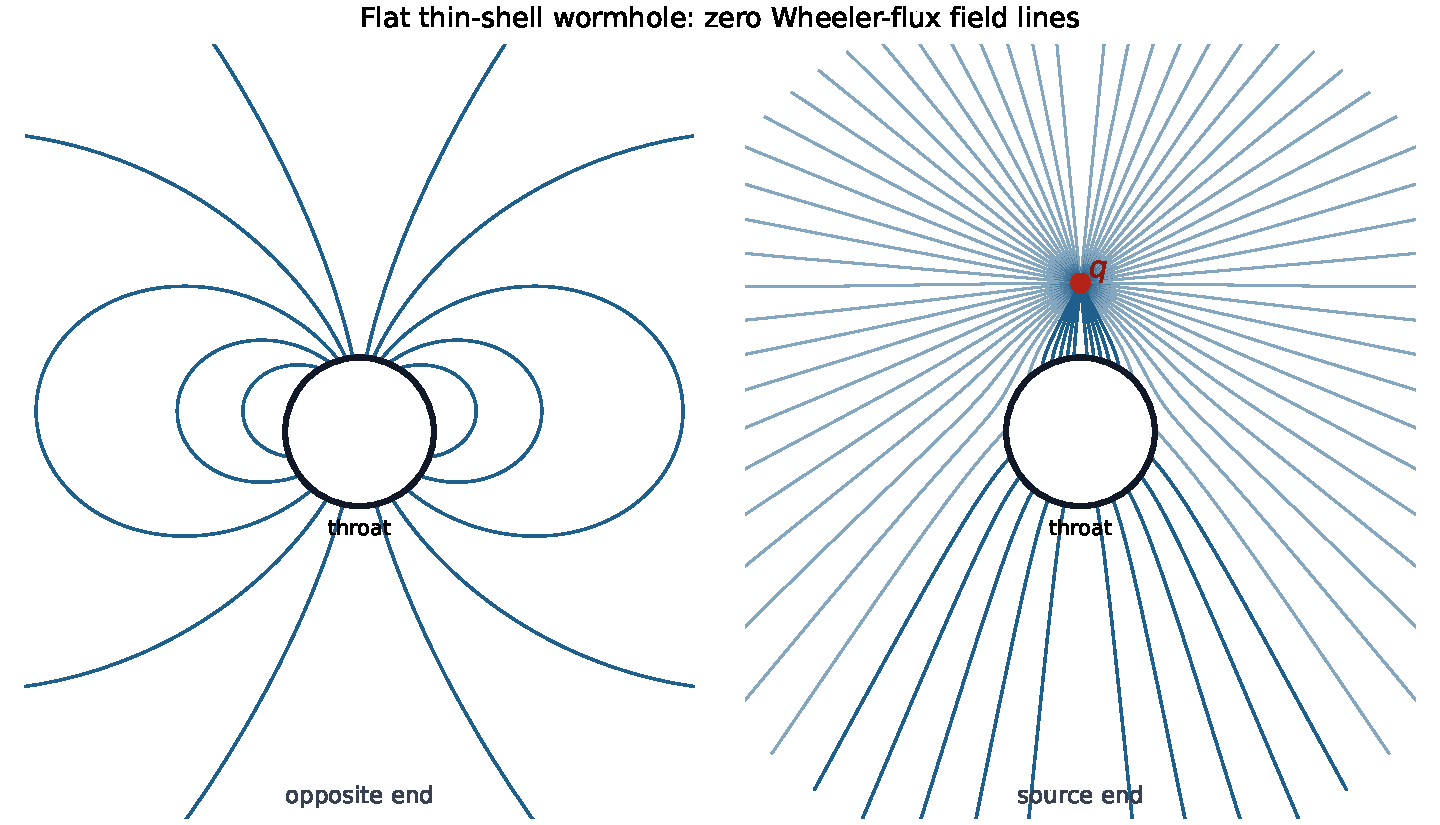
\includegraphics[width=0.95\textwidth]{fig_thinshell_zero_flux_field.pdf}
\caption{\label{fig:thin-shell-zero-flux}
Calculated field-line contours for a point charge near a flat spherical
thin-shell wormhole in the fixed $Q_{\rm wh}=0$ sector.  Each panel is an
ordinary Euclidean exterior chart for one asymptotic end; the black circle is
the same glued throat sphere in the two charts.  Dark blue contours are
throat-detouring flux tubes: they cross the glued sphere in one angular band
and cross back in another.  Complete source-generated tubes still connect the
charge to the source-side infinity.}
\end{figure}

The Dai--Stojkovic signal needs the observed $1/r$ coefficient at one mouth to
vary as the source moves on the other side.  Maxwell theory forbids that
electric monopole response by Stokes' theorem.  Two-ended gravity has the
analogous conservation of the two ADM end charges.  In single-ended
gravity, where there is no per-mouth ADM charge, the exact nonlinear statement
is quasi-local: the Brown--York throat energy of a worldtube enclosing the
throat can change only if stress-energy crosses the worldtube or Brown--York
boundary work is done by changing the worldtube geometry.

Source motion confined to one side cannot produce that signal unless current
or stress-energy crosses the throat worldtube, or Brown--York boundary work
acts on it.  When that happens, the effect is flux/backreaction.

\begin{figure}[!t]
\centering
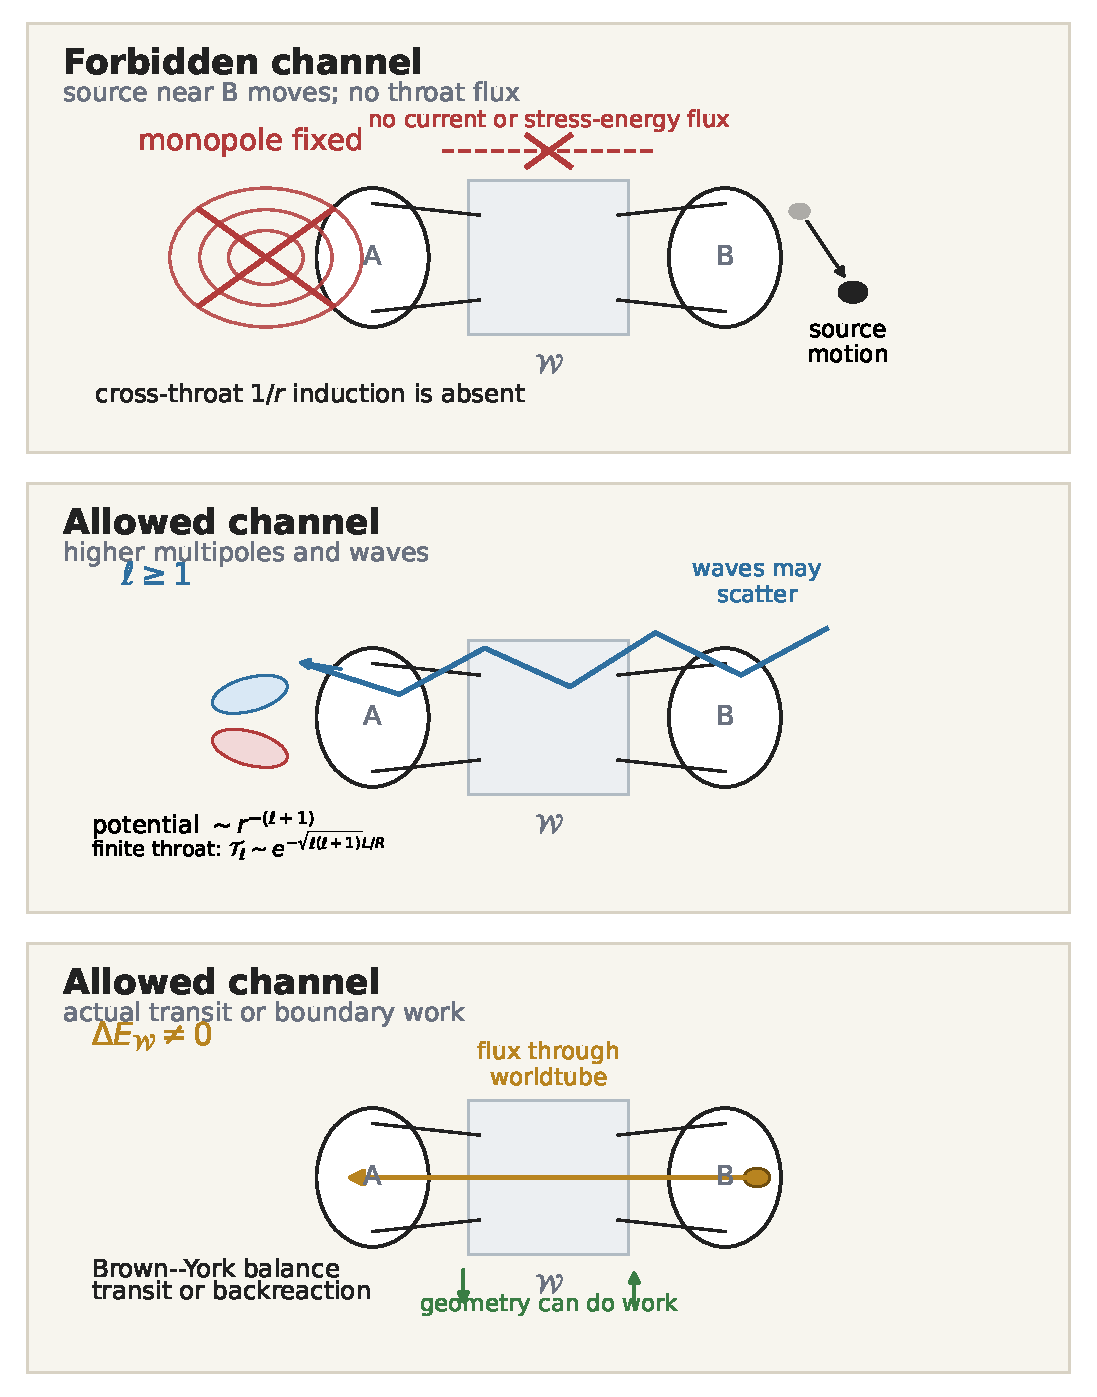
\includegraphics[width=0.86\textwidth]{fig_channel_schematic.pdf}
\caption{\label{fig:channel-schematic}
Response channels for a source near mouth B and an observer near mouth A.
With no current or stress-energy flux through the throat worldtube
$\mathcal W$, and no Brown--York boundary work in the gravitational case,
cross-throat $1/r$ induction is absent.  Higher multipoles and waves may
propagate or scatter through the geometry, but they are not the conserved
monopole channel.
Transit, or Brown--York boundary work, can change the Brown--York throat
energy, producing the backreaction channel.  Figure~\ref{fig:thin-shell-zero-flux}
shows the Maxwell field-line response at fixed throat flux.}
\end{figure}

We assume that traversable wormholes are admissible geometries.  This is a
strong assumption.  Such spacetimes lie outside the hypotheses of standard
topological censorship; in asymptotically flat general relativity they require
violations of the averaged null energy condition or modified dynamics
\cite{FriedmanSchleichWitt1993TopologicalCensorship,MorrisThorne1988Wormholes,
MorrisThorneYurtsever1988TimeMachines,Visser1995LorentzianWormholes}.  The
claims below are conditional on their existence.

The Maxwell result of Sec.~\ref{sec:maxwell} is the local worldtube form of
Frolov and Novikov's electromagnetic flux conservation
\cite{FrolovNovikov1990PhysicalEffects}, restated in spacetime-Stokes form for
a surface around a chosen mouth; the homological framing in
Appendix~\ref{app:cohomology} follows their Sec.~IV.  Krasnikov later applied
related fixed-flux reasoning to electrostatic wormhole interactions and used
Birkhoff's theorem to rule out the spherically symmetric gravitational version
of the Dai--Stojkovic signal
\cite{Krasnikov2008ElectrostaticInteraction,Krasnikov2020CommentObserving}.
The argument below does not assume spherical symmetry.  Maxwell theory supplies
the fixed-flux prototype; the gravitational sections then treat the ADM,
Brown--York, Komar, and linearized quantities used in the observational
proposal.

We distinguish asymptotic charges from local mouth coefficients, and conserved
sectors from response channels.  The Maxwell calculation gives the fixed-flux
result and the fixed-potential contrast.  The gravitational part uses ADM end
charges, Brown--York throat balance, and Komar or linearized
charges.  The final sections return to Dai--Stojkovic, transit/backreaction,
and observational scalings.
Unless stated otherwise, we use geometrized units $G=c=1$.  When quoting
numerical estimates in SI units, we restore the appropriate powers of $G$ and
$c$.

%% ============================================================
\section{Mouth Quantities and Field Sectors}
\label{sec:quantities}
%% ============================================================

The phrase ``mass of a wormhole mouth'' hides three different quantities.  The
distinction matters because the Dai--Stojkovic mechanism requires a local
$1/r$ coefficient to change in response to source motion at the other mouth.
Below, a ``sector'' is a class of field data with the same conservation or
propagation behavior, while a ``channel'' is a physical mechanism that can
produce a response.  The same distinctions are used first in Maxwell theory and
then in the gravitational problem.

By an asymptotically flat end we mean a connected region of a spatial slice
outside a compact set on which the metric approaches the flat metric with the
usual falloff
\cite{ArnowittDeserMisner1962Dynamics,ReggeTeitelboim1974SurfaceIntegrals,
Bartnik1986Mass}.  For Hamiltonian statements involving ADM charges, we use
the Regge--Teitelboim asymptotic class: in asymptotically Cartesian
coordinates, $h_{ij}-\delta_{ij}=O(r^{-1})$ and $\pi^{ij}=O(r^{-2})$, with the
usual parity conditions that make the ADM surface terms finite and
differentiable.  A two-ended wormhole has two such asymptotic regions;
asymptotic charges are then defined separately at the two ends.  A
single-ended wormhole has both mouths in the same asymptotically flat region,
so there is only one asymptotic infinity and no per-mouth ADM charge.

\subsection{Asymptotic charge}

On an asymptotically flat end, the coefficient of the $1/r$ term in the metric
or electromagnetic potential is an asymptotic boundary charge: ADM mass,
ADM momentum, or total electric charge.  If a spacetime has several
asymptotic ends, these charges are defined end by end.  They are not local
properties of a finite mouth; they are charges measured at infinity in the
chosen end.

\subsection{\texorpdfstring{Mouth $1/r$ coefficient}{Mouth 1/r coefficient}}

In a single-ended wormhole, both mouths lie in the same asymptotically flat
universe.  There is only one ADM mass at infinity, so a per-mouth ADM charge is
not available.  Nevertheless, in a source-free region between enclosing spheres
around one mouth one can often expand the field in spherical harmonics and
speak of a local Coulomb/Newtonian $1/r$ coefficient.  The radial variable $r$
is the radius in this local source-free expansion around the chosen mouth; the
expansion is meant on scales large compared with the mouth and before other
sources are enclosed.  This local coefficient is the Dai--Stojkovic observable.
We use it only in settings where it has a charge interpretation:
Maxwell theory, stationary vacuum gravity with Komar integrals, and linearized
gravity with a nonradiative $\ell=0$ constraint charge.

\subsection{Throat energy}

For fully nonlinear single-ended gravity, the finite-region quantity used below
is the quasi-local energy on a timelike worldtube enclosing the throat.  The
Brown--York boundary stress tensor is
\cite{BrownYork1993Quasilocal,Szabados2009Quasilocal}
\begin{equation}
  \tau^{ab}
  =
  \frac{1}{8\pi}\left(K^{ab}-K\gamma^{ab}\right)
  -\tau_{\rm ref}^{ab},
\end{equation}
where $\gamma_{ab}$ is the induced metric on $\mathcal W$, $K_{ab}$ is the
extrinsic curvature of $\mathcal W$ in spacetime, and $\tau_{\rm ref}^{ab}$ is
the boundary stress from the chosen reference functional.  From here on,
$\tau^{ab}$ denotes this subtracted stress tensor.

For a section $S_t\subset\mathcal W$, define
\begin{equation}
  E_{\mathcal W}[\xi;t]
  =
  \int_{S_t}\tau_{ab}u^a\xi^b\,dS,
\end{equation}
where $t$ labels the foliation of $\mathcal W$ generated by the chosen boundary
time flow $\xi^a$, $S_t$ is the associated two-dimensional spatial
cross-section, and $u^a$ is the future unit normal to $S_t$ within
$\mathcal W$.  The shaded throat worldtube in
Fig.~\ref{fig:channel-schematic} represents this $\mathcal W$.  We call
$E_{\mathcal W}$ the Brown--York throat energy.  It is a quasi-local
Hamiltonian boundary charge, not automatically the observed $1/r$ coefficient
in a dynamical exterior.

The same reference functional of the boundary metric is used whenever
different sections of $\mathcal W$ are compared.  If the reference functional
is diffeomorphism invariant, its boundary stress is covariantly conserved on
$\mathcal W$.  Under the no-work condition $\mathcal L_\xi\gamma_{ab}=0$, the
reference term gives no independent change in $E_{\mathcal W}[\xi;t]$.

\subsection{Three field sectors}

We distinguish three field sectors.  Only the last two are genuine response
channels; the first is the conserved sector that cross-throat monopole
induction would have to change.
\begin{itemize}
\item \emph{Conserved monopole sector.}  This is the long-range $\ell=0$ or
$1/r$ coefficient: the handle flux $Q_{\rm wh}$ in Maxwell theory on a
single-ended handle, the ADM charge of an asymptotic end in two-ended gravity,
and a Komar or linearized constraint charge in stationary or linearized
gravity.  In fully nonlinear single-ended gravity the exact finite-region
object is the Brown--York throat energy.  Source motion near the other mouth
cannot change this sector without flux through the worldtube or boundary work.
\item \emph{Propagating sector.}  This consists of higher multipoles and waves.
These terms may depend on source position and motion.  Their large-radius behavior is
different from the unsuppressed $1/r$ signal: a static $\ell\ge1$ multipole has
potential falloff $r^{-(\ell+1)}$ and field falloff $r^{-(\ell+2)}$.
\item \emph{Flux/backreaction sector.}  This consists of current or
stress-energy crossing the throat worldtube, or Brown--York boundary work on
that worldtube.  For Maxwell theory this means electric current crossing a
worldtube or handle cut.  For Brown--York throat energy it means stress-energy
crossing the throat worldtube or boundary work from time-dependent worldtube
geometry.
\end{itemize}

%% ============================================================
\section{Maxwell Theory: Fixed Flux Versus Fixed Potential}
\label{sec:maxwell}
%% ============================================================

Maxwell theory on a fixed wormhole background isolates the sector issue without
gravitational ambiguity.  Frolov and Novikov derived integral conservation laws
for electromagnetic fluxes in multiply connected wormhole spacetimes.  In
particular, exterior charge motion does not change the wormhole flux unless
charged particles pass through the handle
\cite{FrolovNovikov1990PhysicalEffects}.  Krasnikov later used the same
fixed-sector idea in the electrostatic point-charge problem
\cite{Krasnikov2008ElectrostaticInteraction}.  The local worldtube form below
separates quasistatic histories from static families that change the harmonic
sector.

Let $F$ be the Maxwell field and $j$ the current.  Maxwell's equations give
\begin{equation}
  dF=0,\qquad d\star F=4\pi \star j.
\end{equation}
The argument is four-dimensional.  Let $S_t$ be a smooth one-parameter
family of closed two-surfaces, and let
$\mathcal T=\bigcup_{t\in[t_1,t_2]}S_t$ be the three-surface swept out by this
family.  The boundary of $\mathcal T$ consists only of the two endpoint
surfaces, with opposite orientations.  Applying Stokes' theorem to
$d\star F=4\pi\star j$ on $\mathcal T$ relates the change of flux through the
endpoint surfaces to the current flux through $\mathcal T$.

The conservation law concerns the spacetime history of the measuring surface,
not a spatial volume bounded by $S_t$.  The surfaces $S_t$ need not be
separating surfaces in the spatial slice: they need not bound a compact ball
or isolate an asymptotic end.  Additional handles or asymptotic ends may give
additional flux sectors, but they do not allow a chosen sector to change
without current flux through its own swept worldtube.  Conservation applies to
each chosen flux sector, not only to a sum over all mouths or ends.

Applied to the Dai--Stojkovic setup, a surface surrounding the opposite mouth
does not have to be completed by a second surface around the source mouth.  Its
flux is conserved unless electric current crosses its own swept worldtube.
This gives the following local form.

\begin{theorem}[Maxwell flux rigidity]
\label{thm:maxwell-flux}
Let $S_t$ be a smooth family of closed two-surfaces in a wormhole spacetime,
and let $\mathcal T=\bigcup_{t\in[t_1,t_2]}S_t$ be the three-surface they sweep
out between times $t_1$ and $t_2$.  If the net current flux through
$\mathcal T$ vanishes,
\begin{equation}
  \int_{\mathcal T}\star j=0 ,
\end{equation}
then
\begin{equation}
  \int_{S_{t_2}}\star F=\int_{S_{t_1}}\star F .
\end{equation}
\end{theorem}

\begin{proof}
Orient $\mathcal T$ compatibly with the future-directed parameter $t$.  Then
\begin{equation}
  \partial\mathcal T=S_{t_2}-S_{t_1}.
\end{equation}
Integrating $d\star F=4\pi\star j$ over $\mathcal T$ gives
\begin{equation}
  \int_{S_{t_2}}\star F-\int_{S_{t_1}}\star F
  =
  4\pi\int_{\mathcal T}\star j .
\end{equation}
The right-hand side is the electric current crossing the swept worldtube.  If
that current flux vanishes, the two surface fluxes are equal.  No step assumes
that any individual $S_t$ bounds a compact spatial region.
\end{proof}

This local worldtube version is Frolov--Novikov's homological flux law for
closed two-surfaces in a multiply connected spacetime, written for the surface
surrounding a chosen mouth
\cite{FrolovNovikov1990PhysicalEffects}.

Here $S_t$ is the measuring surface and $\mathcal T$ is its history, as drawn
in Fig.~\ref{fig:worldtube-stokes}.  A charge
elsewhere in the spacetime changes the source-dependent field, but not this
flux, unless its worldline, or more generally its current support, crosses
$\mathcal T$.

\begin{figure}[!ht]
\centering
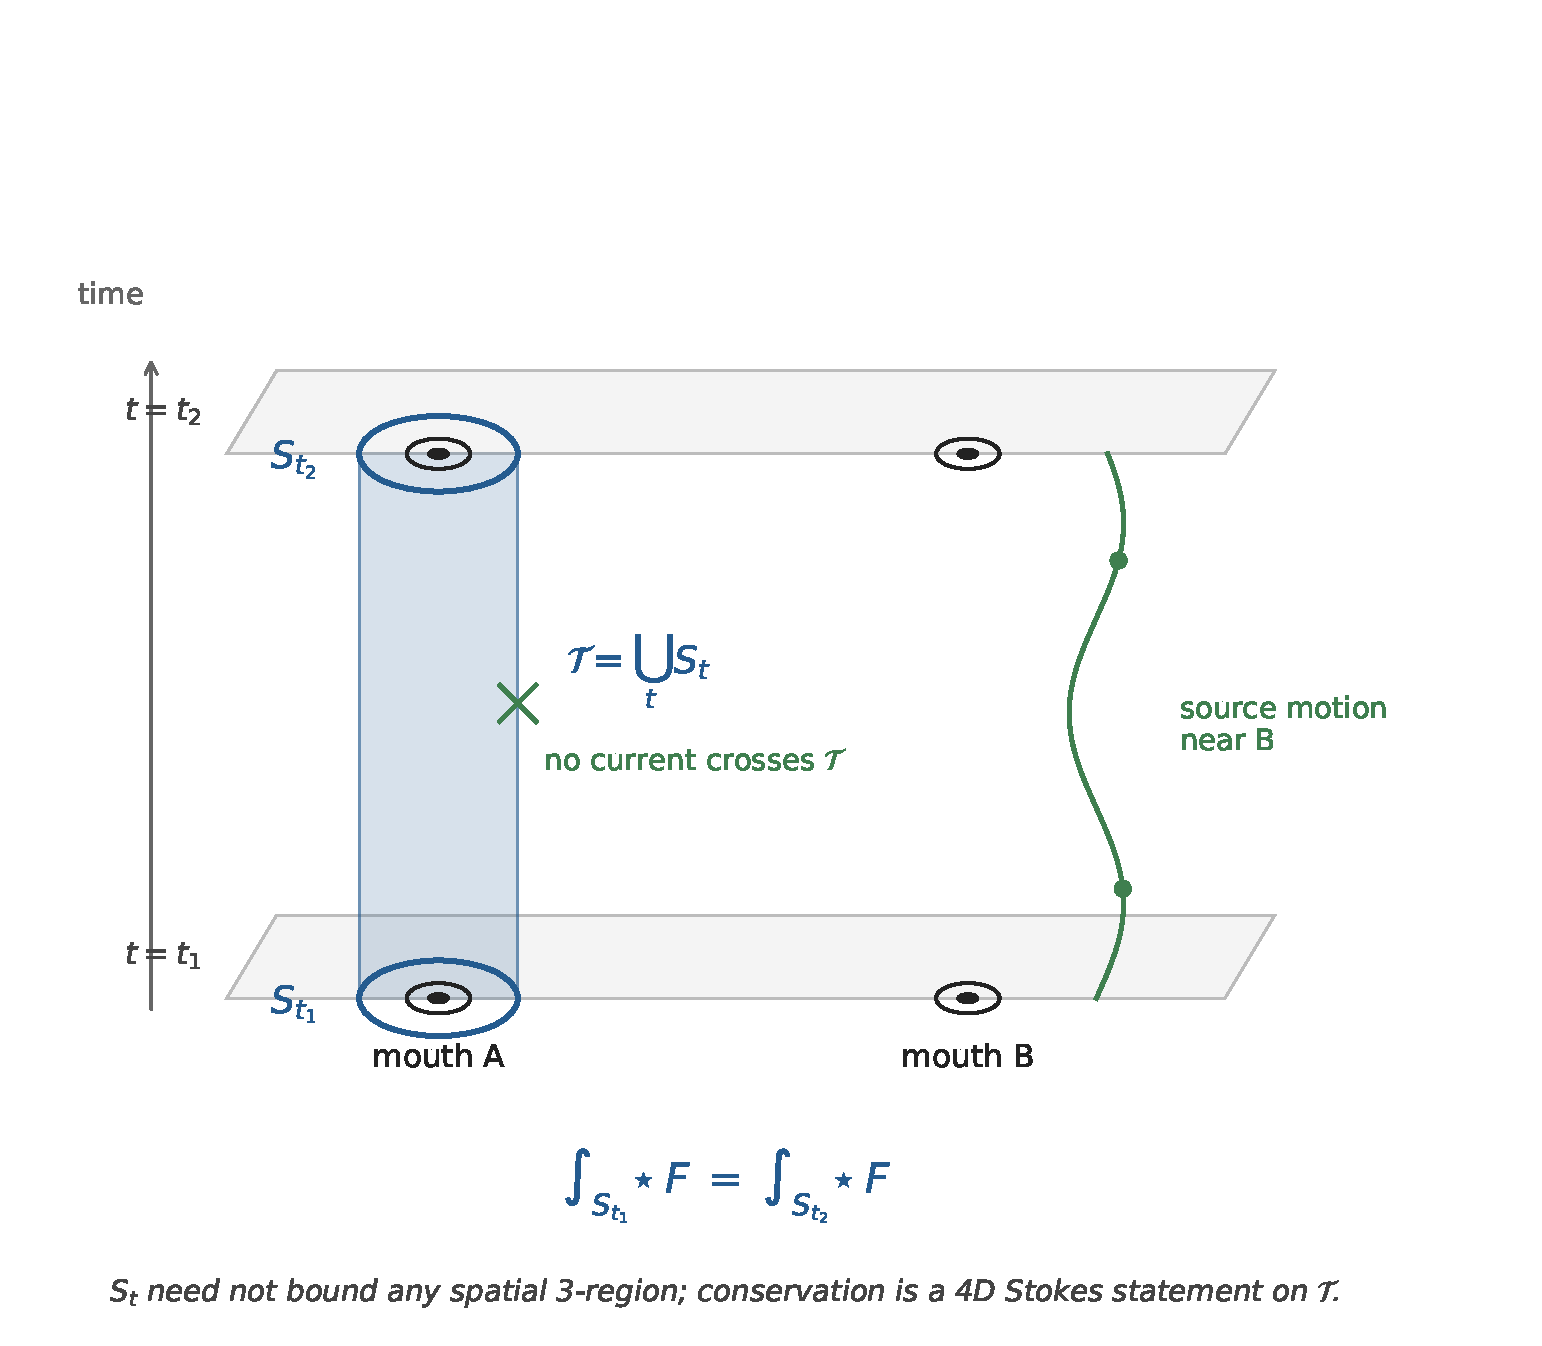
\includegraphics[width=0.75\textwidth]{fig_worldtube_stokes.pdf}
\caption{\label{fig:worldtube-stokes}
Schematic of the Maxwell worldtube argument.  The blue loop represents a closed
two-surface $S_t$ around mouth A, drawn as a loop after suppressing one spatial
dimension.  The flux is compared on the endpoint surfaces $S_{t_1}$ and
$S_{t_2}$ by applying Stokes' theorem to the spacetime history
$\mathcal T=\cup_t S_t$, not to a spatial ball.  Motion near mouth B does not
change this flux unless electric current crosses $\mathcal T$; no auxiliary
surface around mouth B is required.}
\end{figure}

\begin{corollary}[Two-ended Maxwell charges]
On a two-ended wormhole, the electric charge measured at each asymptotic end is
fixed under any evolution in which no current crosses the worldtube swept out
by the asymptotic spheres in that end.
\end{corollary}

\begin{proof}
Take $S_t$ to be a large sphere in the chosen asymptotic end and then let its
radius tend to infinity.
\end{proof}

\begin{corollary}[Single-ended handle flux]
\label{cor:maxwell-handle}
On a single-ended wormhole with a handle, let $S$ be a two-sphere cutting the
handle and define
\begin{equation}
  Q_{\rm wh}:=\frac{1}{4\pi}\int_S\star F .
\end{equation}
The same flux may be measured on any surface homologous to $S$ through a
source-free region, including a surface surrounding the mouth.
If the current support is disjoint from the worldtube swept out by $S$, then
$Q_{\rm wh}$ is conserved.
\end{corollary}

\begin{proof}
Apply Theorem~\ref{thm:maxwell-flux} to the fixed cut surface.  A
localized source moving near one mouth does not intersect this worldtube.  A
charge that actually transits the handle does intersect it, and then the
right-hand side is the transported charge.
\end{proof}

For the single-ended observational topology, Corollary~\ref{cor:maxwell-handle}
is the Maxwell no-induction statement.  A source moving near one mouth changes
higher multipoles, but it does not change the source-free $\ell=0$ handle
sector unless charge actually threads the handle.

\subsection{Two static families}
\label{sec:maxwell-two-families}

Let $X$ denote a source position.  A physical quasistatic family has the
schematic form
\begin{equation}
  \big(F_X,\rho_X;Q_{\rm wh}\big),
  \qquad Q_{\rm wh}\ \hbox{fixed},
\end{equation}
with a gauge choice such as $\Phi_+(\infty)=0$.  In that family the far-end
Coulomb coefficient is fixed by Corollary~\ref{cor:maxwell-handle}.  The
source-dependent field can still change the potential by an additive plateau at
the charge-free end, as in Fig.~\ref{fig:thin-shell-zero-flux-potential}; this
is a voltage offset, not a new far-end electric monopole.

A different family is obtained by imposing Dirichlet data at both infinities for
each $X$,
\begin{equation}
  \Phi_+(\infty)=0,\qquad \Phi_-(\infty)=0 .
\end{equation}
Those two endpoint conditions generally force the homogeneous harmonic
representative to be adjusted as $X$ changes.  This family is a legitimate
sequence of elliptic static problems, but it is not the quasistatic
history of one initial datum unless current crosses the handle and changes
$Q_{\rm wh}$.  Maxwell theory makes the distinction explicit: a wormhole may
carry a source-free Coulomb sector, but that sector is a label, not a response
mode.  Appendix~\ref{app:cohomology} gives the homological form of this
distinction.

\FloatBarrier

%% ============================================================
\section{Gravity: ADM Rigidity and Brown--York Balance}
\label{sec:gravity}
%% ============================================================

The observational proposal is gravitational: source motion near one mouth would
have to create the Newtonian $1/r$ signal read at the other.  Gravity does not
have a Maxwell-like, gauge-invariant flux through an arbitrary closed
two-surface whose value is automatically a conserved monopole charge.  At an
asymptotically flat end, however, the Hamiltonian charge associated with an
asymptotic time translation is the ADM mass, so a two-ended spacetime has
separate ADM Hamiltonians for the two ends.  A finite surface around a mouth in
a single-ended wormhole is different, because it is not an ADM boundary.  The
finite-boundary quantity used below is the Brown--York throat energy
$E_{\mathcal W}$ on a timelike worldtube enclosing the throat.  Its balance law
contains both stress-energy flux and boundary work.  Only in stationary or
linearized regimes can this throat statement be related to the local mouth
$1/r$ coefficient used in the Dai--Stojkovic observable.

Two cases have to be kept apart.  In a two-ended spacetime, the exact monopole
charges are the ADM charges at the two asymptotic ends, and these charges are
conserved end by end.  In a single-ended wormhole, there is no per-mouth ADM
charge, so the nonlinear balance law lives on a finite worldtube around the
throat.  Relating that worldtube charge to a local mouth coefficient then
requires an additional stationary or perturbative argument; it is not an ADM
theorem.

\subsection{Separate ADM charges at distinct ends}

In a spacetime with two asymptotically flat ends $E_+$ and $E_-$, the ADM
charges are defined separately at the two infinities.  Regge--Teitelboim
Hamiltonian evolution makes this separation explicit: an asymptotic time
translation at one end has its own surface Hamiltonian at that end
\cite{ReggeTeitelboim1974SurfaceIntegrals}.  This is the standard end-by-end
assignment of ADM energy-momentum for multi-ended asymptotically flat initial
data
\cite{ArnowittDeserMisner1962Dynamics,Wald1984GeneralRelativity,Bartnik1986Mass}.

\begin{theorem}[Per-end ADM rigidity]
\label{thm:adm-rigidity}
Consider Hamiltonian evolution in general relativity, with matter fields
allowed, on an asymptotically flat two-ended initial data set in the
Regge--Teitelboim class specified in Sec.~\ref{sec:quantities}.  If the
evolution preserves those asymptotic structures, the ADM mass at each end is
separately conserved.
\end{theorem}

\begin{proof}
Choose a smooth lapse $N_+$ that is exactly one on the far region of $E_+$ and
exactly zero on the far region of $E_-$, with all derivatives supported in a
compact interpolation region.  The Regge--Teitelboim improved Hamiltonian is
\begin{equation}
  H[N_+,0]=\int_\Sigma N_+\mathcal H\,d^3x+B[N_+,0],
\end{equation}
where $B$ is the asymptotic surface term.  On the constraint surface the bulk
term vanishes.  Because $N_+$ is exactly constant on each far end, the only
asymptotic surface term is the standard ADM energy of $E_+$; the compact
interpolation region produces no boundary term.  Thus $H[N_+,0]=M_+^{\rm ADM}$
on shell.

The same construction gives $H[N_-,0]=M_-^{\rm ADM}$ on shell.  The
hypersurface-deformation algebra~\cite{HojmanKucharTeitelboim1976Geometrodynamics}
shows that the two asymptotic translations are independent.  Indeed,
\begin{equation}
  \{H[N_+,0],H[N_-,0]\}=H[0,\beta^i],
  \qquad
  \beta^i=h^{ij}(N_+\partial_jN_- - N_-\partial_jN_+).
\end{equation}
Since the lapse gradients have compact support, $\beta^i$ has compact support.
The corresponding momentum-constraint generator has no asymptotic surface
charge and vanishes weakly on the constraint surface.  Hence the end
Hamiltonians commute weakly.  Within the Regge--Teitelboim asymptotic class,
an admissible time evolution has a lapse approaching fixed constants $c_+$ and
$c_-$ at the two ends, plus lapse and shift remainders whose falloff and parity
give no asymptotic surface Hamiltonian.  On the constraint surface those
remainders are proper gauge generators, fixing the asymptotic charges.  Thus
the evolution is weakly equivalent, for the
end energies, to the fixed linear combination
$c_+H[N_+,0]+c_-H[N_-,0]$.  Therefore each selected ADM mass is constant along
such an evolution.
\end{proof}

This theorem concerns asymptotic charges, not finite-region energy.  Even if
matter transits the interior, the ADM mass selected by a fixed asymptotic time
translation does not change.  Transit can change quasi-local or throat
quantities, but not the conserved end charge.

\subsection{Brown--York worldtube balance}

For a single-ended wormhole there is no separate ADM mass for each mouth.  To
state a local throat result, we use the Brown--York stress tensor from
Sec.~\ref{sec:quantities} on a timelike worldtube $\mathcal W$ enclosing the
throat.  Let $n^\mu$ be the outward spacelike unit normal to $\mathcal W$.
Recall the Brown--York charge $E_{\mathcal W}[\xi;t]$ from
Sec.~\ref{sec:quantities}.  Let $\Delta\mathcal W$ denote the portion of
$\mathcal W$ between $S_{t_1}$ and $S_{t_2}$.  The orientation is chosen so
that Stokes' theorem on $\Delta\mathcal W$ gives the future boundary
contribution $E_{\mathcal W}[\xi;t_2]$ and the past boundary contribution
$-E_{\mathcal W}[\xi;t_1]$.

\begin{theorem}[Brown--York worldtube balance]
\label{thm:BY-balance}
Let $\xi^a$ be the time flow used to define $E_{\mathcal W}$ in
Sec.~\ref{sec:quantities}.  Then
\begin{equation}
\label{eq:BY-balance}
  E_{\mathcal W}[\xi;t_2]-E_{\mathcal W}[\xi;t_1]
  =
  \int_{\Delta\mathcal W}
  \left(
    -T_{\mu\nu}n^\mu\xi^\nu
    +\frac12\tau^{ab}\mathcal L_\xi\gamma_{ab}
  \right)d^3V .
\end{equation}
\end{theorem}

\begin{proof}
The Brown--York momentum constraint on the timelike boundary is
\cite{BrownYork1993Quasilocal,EppMcGrathMann2013Momentum}
\begin{equation}
  D_a\tau^{ab}=-T_{\mu\nu}n^\mu\gamma^{\nu b},
\end{equation}
where $D_a$ is the Levi-Civita connection of $\gamma_{ab}$.  Contracting with
$\xi_b$ gives
\begin{equation}
  D_a(\tau^{ab}\xi_b)
  =
  -T_{\mu\nu}n^\mu\xi^\nu+\tau^{ab}D_a\xi_b.
\end{equation}
Since $\tau^{ab}$ is symmetric,
\begin{equation}
  \tau^{ab}D_a\xi_b=\frac12\tau^{ab}\mathcal L_\xi\gamma_{ab}.
\end{equation}
Integrating this identity over the slab $\Delta\mathcal W$ and applying
Stokes' theorem on $\Delta\mathcal W$ gives \eqref{eq:BY-balance}.  Since
$\Delta\mathcal W$ is a slab of the timelike boundary itself, its intrinsic
boundary is $S_{t_2}-S_{t_1}$; there is no lateral contribution.
\end{proof}

\begin{corollary}[No-flux/no-work throat rigidity]
\label{cor:zero-flux}
If
\begin{equation}
  T_{\mu\nu}n^\mu\xi^\nu=0,
  \qquad
  \mathcal L_\xi\gamma_{ab}=0
\end{equation}
on $\Delta\mathcal W$, then
\begin{equation}
  \Delta E_{\mathcal W}[\xi]=0.
\end{equation}
\end{corollary}

\begin{proof}
Both terms in the integrand of \eqref{eq:BY-balance} vanish.
\end{proof}

\begin{corollary}[Outgoing flux with no work]
\label{cor:outgoing-flux}
With $n^\mu$ oriented outward from the enclosed throat region and with
$\mathcal L_\xi\gamma_{ab}=0$, positive stress-energy flux leaving that region
decreases the Brown--York throat energy:
\begin{equation}
  T_{\mu\nu}n^\mu\xi^\nu>0
  \quad\Longrightarrow\quad
  \Delta E_{\mathcal W}[\xi]<0 .
\end{equation}
\end{corollary}

\begin{proof}
With $\mathcal L_\xi\gamma_{ab}=0$,
\begin{equation}
  \Delta E_{\mathcal W}[\xi]
  =
  -\int_{\Delta\mathcal W}T_{\mu\nu}n^\mu\xi^\nu\,d^3V .
\end{equation}
The integrand is positive by hypothesis, so the change in
$E_{\mathcal W}[\xi]$ is negative.
\end{proof}

The second term in \eqref{eq:BY-balance} has no Maxwell analogue.  It is a
stress-times-strain term: the Brown--York boundary
stress contracted with the change of the worldtube metric along the chosen time
flow.  It is the finite-boundary analogue of pressure-volume work.  A vacuum
region can exchange Brown--York throat energy by changing boundary geometry
even when no ordinary matter crosses the boundary.  The gravitational
counterpart of Maxwell worldtube rigidity has two parts: no stress-energy flux
through $\mathcal W$, and no Brown--York boundary work,
$\tau^{ab}\mathcal L_\xi\gamma_{ab}=0$, from changing induced geometry on
$\mathcal W$.

\begin{remark}[Dynamical throat response]
\label{rem:dynamical-throat-response}
A time-dependent perturbation can also act on the matter or geometry supporting
the throat.  If this changes the induced worldtube metric, then
$\mathcal L_\xi\gamma_{ab}\ne0$ and the Brown--York work term in
\eqref{eq:BY-balance} contributes even when no stress-energy flux crosses
$\mathcal W$.  Such a process is backreaction, not cross-throat monopole
induction.  Its size and sign depend on the
throat-support model and boundary conditions.
\end{remark}

%% ============================================================
\section{Exterior Mouth \texorpdfstring{$1/r$}{1/r} Field}
\label{sec:mouth-bridge}
%% ============================================================

Corollary~\ref{cor:zero-flux} controls the finite throat quantity: the
Brown--York Hamiltonian boundary charge associated with the chosen time flow
$\xi^\mu$ on the throat worldtube.  The Dai--Stojkovic observable is not this
Brown--York throat energy, but an exterior mouth $1/r$ coefficient.  A link
between them requires a regime in which the exterior coefficient is a conserved
or constraint charge.

\subsection{Stationary vacuum exterior}

\begin{theorem}[Stationary-vacuum Komar equality]
\label{thm:komar-propagation}
Let $U_A$ be a stationary vacuum shell, topologically $S^2\times I$ with $I$
an interval bounded by the two spheres, between an inner sphere $S_{\rm in}$
around mouth $A$ and a larger sphere $S_R$ in the local far zone of that
mouth.  Suppose $U_A$ admits a timelike Killing field
$\xi^\mu$, normalized to the stationary time coordinate used to read off the
local weak-field Newtonian potential.  Define
\begin{equation}
  M_K[S]=-\frac{1}{8\pi}\int_S\star d\xi^\flat .
\end{equation}
If $M_K[S_{\rm in}]$ is fixed, then the stationary gravitational $1/r$
coefficient measured at $S_R$ is fixed.
\end{theorem}

\begin{proof}
For a Killing field in vacuum,
\begin{equation}
  d\star d\xi^\flat=-2\star(R_{\mu\nu}\xi^\nu dx^\mu)=0 .
\end{equation}
Thus $\star d\xi^\flat$ is closed, and Stokes' theorem gives
$M_K[S_R]=M_K[S_{\rm in}]$ because $S_R$ and $S_{\rm in}$ bound the shell $U_A$
\cite{Komar1959Covariant}.  With $\xi^\mu$ normalized as above, $M_K[S_R]$ is
the standard Komar normalization of the stationary gravitational $1/r$
coefficient read off at $S_R$.  A fixed inner Komar integral therefore implies
a fixed exterior mouth $1/r$ coefficient.
\end{proof}

This is only a statement about the stationary vacuum shell.  It does not
identify the finite Brown--York throat energy with Komar mass.  The Komar
argument says that once the inner Komar integral is fixed, the same value is
read on the outer sphere where the $1/r$ coefficient is measured.

\begin{lemma}[Conditional Brown--York-to-Komar implication]
\label{lem:BY-komar}
Assume the setup of Theorem~\ref{thm:komar-propagation}.  Suppose the
Brown--York work term vanishes on the throat worldtube,
\begin{equation}
  \mathcal L_\xi\gamma_{ab}=0,
\end{equation}
and suppose the stationary vacuum boundary-value problem in $U_A$, with the
induced stationary boundary data on the worldtube and the chosen normalization
of $\xi^\mu$, has a unique solution up to diffeomorphisms fixed on the
boundary.  Then the inner Komar integral is fixed, and hence the observed mouth
$1/r$ coefficient is fixed.
\end{lemma}

\begin{proof}
The no-work condition says that the boundary metric is invariant under the
chosen time flow $\xi$.  The inner boundary data supplied to the stationary
exterior is therefore the same at each time.  By the stated uniqueness
assumption, the full stationary vacuum exterior solution is the same, up to a
boundary-fixing diffeomorphism.  In particular the
exterior limit of $\nabla_\mu\xi_\nu$ at $S_{\rm in}$, including the normal
derivative entering $\star d\xi^\flat$, is fixed.  The Komar integral is built
from that exterior solution and is diffeomorphism invariant, so
$M_K[S_{\rm in}]$ is fixed.  Theorem~\ref{thm:komar-propagation} then gives the
same value on $S_R$.
\end{proof}

The uniqueness assumption in Lemma~\ref{lem:BY-komar} is part of the hypothesis.
It is the additional input needed to turn fixed stationary worldtube geometry
into a fixed inner Komar integral; the Brown--York balance law alone does not
supply that exterior boundary-value result.  Exterior stationary or static
vacuum uniqueness is known in restricted perturbative settings, for example
near stationary conformally flat exterior data and near round static Bartnik
boundary data
\cite{Klenk1999StationaryVacuumExterior,Anderson2015ExteriorStaticVacuum}.
Lemma~\ref{lem:BY-komar} is therefore only a sufficient-condition bridge from
throat data to the mouth coefficient.  It is not a general uniqueness theorem
for nonlinear stationary exteriors.  The fully dynamical case remains limited
to the Brown--York balance statement.

\subsection{Linearized exterior}

\begin{proposition}[No first-order mouth induction]
\label{prop:linearized}
Consider linearized gravity on a fixed single-ended wormhole background with a
source-free region near mouth $A$, and hold the background throat worldtube
geometry fixed.  Define the first-order mouth $1/r$ coefficient as the nonradiative
$\ell=0$ coefficient of the $1/r$ metric perturbation in that region,
equivalently the linearized Komar/constraint charge on enclosing spheres.  If
the perturbing matter remains on the $B$ side and no stress-energy crosses the
throat worldtube, then this first-order mouth $1/r$ coefficient at $A$ is
constant.
\end{proposition}

\begin{proof}
The linearized Bianchi identity gives a conserved linearized constraint charge
for the nonradiative $\ell=0$ sector.  Equivalently, the linearized Hamiltonian
constraint relates the difference of the $\ell=0$ surface charge on two
enclosing spheres to the matter energy in the spatial shell between them
\cite{ReggeTeitelboim1974SurfaceIntegrals,AbbottDeser1982Stability}.  In the
source-free $A$-mouth region, the surface charge is therefore independent of
which enclosing sphere is used.  Its time change is governed by the
corresponding spacetime conservation law and can be sourced only by
stress-energy flux through the swept worldtube.  By hypothesis there is none.
Linearized gravitational radiation does not supply a radiative monopole
channel; radiative gravitational multipoles begin at $\ell\ge2$
\cite{Thorne1980Multipole}.  The first-order mouth $1/r$ coefficient is
therefore constant.
\end{proof}

\begin{remark}[Radiative nonlinear obstruction]
In a fully nonlinear radiative exterior there need not be a timelike Killing
field, and a finite-radius ``mouth $1/r$ coefficient'' is not a canonical
invariant.  We do not state a fully dynamical mouth-rigidity theorem.  There
the invariant result is the Brown--York worldtube balance law, not a separate
theorem for a finite-radius mouth coefficient.
\end{remark}

For the quasistatic regime contemplated by Dai and Stojkovic, such as the S2
orbit around Sgr~A* with $v/c\sim0.02$, Proposition~\ref{prop:linearized} gives
the no-induction result.  Lemma~\ref{lem:BY-komar} gives the adiabatic
stationary limit.  Slow source motion on the far side does not by itself supply
the flux or boundary work needed to change the conserved $\ell=0$ sector.

%% ============================================================
\section{Application to the Dai--Stojkovic Channel}
\label{sec:ds}
%% ============================================================

Dai and Stojkovic construct a family of static solutions in which the
coefficient assigned to the opposite-side $1/r$ term changes as the source
position is varied \cite{DaiStojkovic2019Observing}.  This elliptic
boundary-value family does not by itself define time evolution of one system
with a fixed conserved flux sector.  The conservation laws above rule out such
a history for the mouth $1/r$ coefficient.

In Maxwell theory, varying the opposite-side Coulomb coefficient changes the
conserved handle flux $Q_{\rm wh}$.  Source motion that does not send charge
through the throat cannot do that.  The only unsuppressed term in the
opposite-side far field is fixed; source-dependent effects begin in
higher multipoles or in radiation.

In the short-throat electrostatic model the sector change is explicit.  The two
sides are matched at the mouth, so the finite-length attenuation discussed in
Sec.~\ref{sec:consequences} is absent.  For a point charge $q$ at distance $A$
from a throat of radius $R$, the Dai--Stojkovic matching prescription, in
which the static potential and normal field are matched at the throat sphere,
gives the opposite-side effective charge
\begin{equation}
  Q_{\rm opp}^{\rm DS}(A)=\frac{qR}{2A}.
\end{equation}
For two source positions $A_0$ and $A_1$, the two static solutions differ by a
source-free harmonic contribution
\begin{equation}
  \Delta Q_{\rm wh}
  =
  \frac{qR}{2}\left(\frac{1}{A_0}-\frac{1}{A_1}\right).
\end{equation}
Following the Dai--Stojkovic curve as a function of source position requires
the harmonic sector itself to drift.
Corollary~\ref{cor:maxwell-handle} forbids that drift unless charge crosses the
handle.  The static family lies in different flux sectors; it is not a
dynamical trajectory of one physical system.  The sector-drift formula places
the Dai--Stojkovic inference in the fixed-flux problem discussed by
Frolov--Novikov and Krasnikov.  This does not depend on finite-throat
attenuation.

Figure~\ref{fig:thin-shell-zero-flux} shows the local content of the
fixed-flux condition: fixing $Q_{\rm wh}$ fixes the oriented integral through
the throat, but it leaves the higher-multipole response intact.

The same distinction appears in the familiar electrostatic problem of a charge
held near a Schwarzschild black hole
\cite{Copson1928Electrostatics,HanniRuffini1973Lines,
Linet1976Electrostatics,PoissonPoundVega2011Motion}.  The external charge
distorts field lines and can be described as inducing a horizon surface-charge
distribution, but this polarization does not by itself change the black hole's
net charge parameter; that changes only when real charge crosses the horizon.
Historically, Copson's solution carried an unphysical extra monopole
contribution, which Linet removed by adding the appropriate homogeneous
monopole solution.  The boundary-value problem has to be placed in the correct
monopole sector.  The Dai--Stojkovic static matching
family has the analogous structure: each source position selects a different
harmonic-flux sector around the opposite mouth, but moving the source through
that family is a change of sector, not a dynamical response generated by source
motion alone.

In the two-ended gravitational setup, the $1/r$ coefficient is the ADM mass at
an asymptotic end.  Theorem~\ref{thm:adm-rigidity} says that this end charge is
separately conserved.  Source motion in the interior cannot modulate it.

In the single-ended gravitational setup, the exact nonlinear result is the
Brown--York no-flux/no-work result, not a per-mouth ADM theorem:
Corollary~\ref{cor:zero-flux} says that no stress-energy flux and no
Brown--York boundary work fix the Brown--York throat energy.  Under the
stationary-vacuum assumptions of Theorem~\ref{thm:komar-propagation} and
Lemma~\ref{lem:BY-komar}, or at first order by
Proposition~\ref{prop:linearized}, the mouth $1/r$ coefficient is also fixed.
A quasistatic perturber on the other side that does not cross the throat cannot
generate the S2-style time-dependent Newtonian $1/r$ coefficient.

Krasnikov's 2020 comment on Dai--Stojkovic used Birkhoff's theorem to rule out
the spherically symmetric gravitational signal in their approximation
\cite{Krasnikov2020CommentObserving}.  The conservation argument here does not
use spherical symmetry.  It tracks the conserved sector directly: the proposed
signal needs a changing exterior $1/r$ coefficient or flux sector, while the
assumed source motion supplies no flux or boundary work.

%% ============================================================
\section{The Allowed Channel: Transit and Backreaction}
\label{sec:transit}
%% ============================================================

Corollary~\ref{cor:zero-flux} still allows changes driven by flux
through the throat.

Frolov and Novikov described how a massive particle passing through a wormhole
changes the effective mass parameters associated with the mouths
\cite{FrolovNovikov1990PhysicalEffects}.  Cramer et al. used the same
backreaction idea to suggest that a mouth accreting matter in a high-density
region could drive the other mouth toward negative effective mass, producing a
distinctive negative-mass lensing signature
\cite{CramerEtAl1995NaturalWormholes}.  In both cases, energy or matter
actually crosses the throat.

The Brown--York balance law is the local balance equation for such processes.
If positive energy leaves the throat region through the worldtube and the
boundary work term vanishes, Corollary~\ref{cor:outgoing-flux} gives
\begin{equation}
  \Delta E_{\mathcal W}[\xi]<0.
\end{equation}
If the boundary geometry changes, the work term must also be included.  A
general sign theorem then requires either a stationary boundary or
model-dependent control of the work term.

The observable in the transit problem is different.  After the crossing, if the
exterior of the exiting mouth settles and the escaped body or radiation is
separated from the mouth, the quantity to compare is the settled mouth $1/r$
coefficient measured on a sphere that encloses the mouth support but excludes
the escaped energy.  Conservation then gives a final-state accounting relation
of the form
\begin{equation}
  \Delta M_{\rm mouth}
  =
  -\frac{E_{\rm out}}{c^2}
  +\frac{E_{\rm in}}{c^2}
  +\Delta M_{\rm support},
\end{equation}
where $\Delta M_{\rm support}$ is shorthand for any compensating change in the
throat support sector: exotic-matter support energy, boundary-work residue,
reference-subtraction change, or junction response.  In the
Frolov--Novikov/Cramer limit of outgoing positive energy with no compensating
incoming or support-sector term, the exiting mouth's settled $1/r$ coefficient
decreases by the escaped energy.  Outgoing gravitational radiation is included
in this final-state accounting in the usual Bondi--Sachs sense
\cite{BondiVanderBurgMetzner1962Gravitational,Sachs1962Asymptotic}.

Radiation transit is the wave analogue.  Electromagnetic
radiation contributes through the matter flux term
$T_{\mu\nu}n^\mu\xi^\nu$.  Gravitational radiation contributes through the
effective radiative stress-energy in an averaged description
\cite{Isaacson1968EffectiveStressTensor}, through the Brown--York work term, or
both.  In a simple settled-mouth estimate, a burst of energy $E$ emerging from
the throat and separating from the mouth gives an observable mouth-memory shift
of order
\begin{equation}
  \Delta M_{\rm mouth}\sim -E/c^2,
\end{equation}
up to radiation, work, and support-sector corrections, represented by the
$\Delta M_{\rm support}$ term above.  This
mouth-memory estimate is distinct from the Dai--Stojkovic signal: it is
driven by real flux through the throat, not by source motion confined to the
other side.

%% ============================================================
\section{Consequences and Limitations}
\label{sec:consequences}
%% ============================================================

\subsection{What is ruled out}

Cross-throat monopole induction is ruled out when the throat worldtube has
no current or stress-energy flux through it and no Brown--York boundary work
on it.  A source staying on the far side of a throat cannot then create a new
time-dependent mouth $1/r$ coefficient in the regimes where that coefficient
is fixed by charge conservation or by the stationary/linearized arguments
above.
The Dai--Stojkovic S2-style observational proposal requires this channel.

\subsection{What remains}

A wormhole can have a pre-existing charge or mass parameter.  Source motion on
the other side does not modulate it; the parameter need not vanish.

Higher multipoles can couple across a throat.  They belong to the
propagating/source-dependent sector, not to the conserved $1/r$ sector.  A
finite throat can attenuate them further.  In an approximately cylindrical
static throat of length $L$ and radius $R$, the transverse spherical harmonic obeys
$k_\ell^2=\ell(\ell+1)/R^2$, so the mode amplitude is suppressed by
\begin{equation}
  \mathcal T_\ell \sim
  \exp\!\left[-\sqrt{\ell(\ell+1)}\,L/R\right].
\end{equation}
Even the dipole carries $\mathcal T_1\sim \exp(-\sqrt2\,L/R)$.  This
is the cylindrical below-cutoff factor of the aperture analogy in
Sec.~\ref{sec:intro}.  The attenuation is separate from the conserved-sector
result; it is an extra penalty on the higher-multipole channels that remain
after the $\ell=0$ sector is removed.

Radiation and matter can cross the throat.  The Brown--York balance law then
permits the Brown--York throat energy to change, matching the
transit/backreaction channel in the older mouth-mass literature.

A fully nonlinear radiative single-ended exterior remains outside the
stationary-vacuum and linearized results above.  The exact statement there is
Brown--York balance, not a theorem for a finite-radius mouth $1/r$
coefficient.

\subsection{Observational implication}

The proposed Sgr~A* signal is a time-varying $1/r^2$ acceleration of S2 sourced
by an object that remains on the other side of a wormhole
\cite{DaiStojkovic2019Observing}.  Simonetti et al. improve the observational
reach by moving the same channel to more sensitive systems
\cite{SimonettiEtAl2021SensitiveSearches}.  The conservation results remove
cross-throat monopole induction.  Dai and Stojkovic already work in the
short-throat limit, where no evanescent decay is present; the limiting point is
the conserved character of the unsuppressed $\ell=0$ coefficient.

The scale of the removed term is the one used in the original Sgr~A* estimate:
$M_{\rm Sgr\,A*}\simeq4\times10^6M_\odot$, gravitational radius
$r_g\simeq0.084\,{\rm AU}$, mouth size $R\sim r_g$, S2 radius
$r_2\sim1000\,{\rm AU}$, and an opposite-side perturber of a few solar masses at a few
$r_g$ \cite{DaiStojkovic2019Observing}.  Their quoted target acceleration
precision is $10^{-6}\,{\rm m\,s^{-2}}$.  Under the conserved-sector
hypotheses, the induced $\ell=0$ term used for that estimate is absent.

Removing the conserved $\ell=0$ response changes what the observation can test.
Source-motion signals must then come from $\ell\ge1$ multipoles or waves.
Their potential falls as
$r^{-(\ell+1)}$ and their field or acceleration falls as $r^{-(\ell+2)}$.  For
a short throat ($L/R\lesssim1$), the dipole is not exponentially suppressed by
the finite-throat factor above, so the leading cost is geometric.  Using the
same Sgr~A* length scales, a mouth-scale dipole carries one extra far-zone
factor
\begin{equation}
  \frac{R}{r_2}\sim \frac{0.084}{1000}\simeq 8.4\times10^{-5}
\end{equation}
relative to a hypothetical monopole of comparable coefficient.  In a finite
cylindrical throat the dipole also carries
$\mathcal T_1=\exp(-\sqrt2\,L/R)$: $\mathcal T_1\simeq8.5\times10^{-4}$ at
$L/R=5$ and $\mathcal T_1\simeq7.2\times10^{-7}$ at $L/R=10$.  These factors do
not apply to the Dai--Stojkovic short-throat idealization, where $L/R$ is
effectively zero; they quantify the additional cost of finite-length
higher-multipole leakage.  Higher multipoles are still more suppressed, both
geometrically and through the throat.  If the removed monopole term were at
the quoted $10^{-6}\,{\rm m\,s^{-2}}$ scale, the leading dipole geometric
factor alone would put an otherwise comparable source-motion signal at
$\sim10^{-10}\,{\rm m\,s^{-2}}$, before any finite-throat attenuation.

For the flux/backreaction channel, a compact-object merger gives a reference
scale.  If a burst with $E_{\rm GW}/c^2\simeq0.5M_\odot$ is emitted on the
source side at distance $D=1\,{\rm pc}$ from a mouth of radius
$R_{\rm th}=10^3\,{\rm m}$, and the intercepted energy is transmitted through
the wormhole and later exits the observer-side mouth, then taking unit coupling
efficiency in an isotropic solid-angle estimate gives the settled mouth-memory
estimate
\begin{equation}
  \Delta M_{\rm mouth}
  \sim
  -\frac{E_{\rm GW}}{c^2}\frac{R_{\rm th}^2}{4D^2}
  \simeq -2.6\times10^2\,{\rm kg}.
\end{equation}
Relative to $4\times10^6M_\odot$ this is $\sim3\times10^{-35}$.  The estimate
uses a small illustrative throat and is not the Dai--Stojkovic horizon-scale
mouth.  The negative sign refers to the final settled mouth $1/r$ coefficient
on a sphere excluding the escaped radiation; incoming radiation, boundary work,
or support-sector response contributes additional terms.
Appendix~\ref{app:backreaction-sign} gives the assumptions and solid-angle estimate
behind this number.

Other wormhole searches probe different channels.  Pre-existing lensing or mass
signatures, wave scattering, echoes, and transit/backreaction involve fixed
background parameters, propagating waves, or real flux through the throat
\cite{BaoHouZhang2023GWScattering,CramerEtAl1995NaturalWormholes}.  Their
assumptions are separate from cross-throat monopole induction.

%% ============================================================
\section{Discussion}
\label{sec:discussion}
%% ============================================================

The preceding sections separate three effects that are easily conflated.
Fields can pass through a throat and return, higher multipoles and waves can
couple across it, and matter or radiation can change the throat by carrying
real flux or doing boundary work.  None of these effects is a modulation of
the conserved monopole sector by source motion on the far side.

The Dai--Stojkovic mechanism fails even in the short-throat limit.  In that
limit there is no finite-length attenuation to blame; the problem is
conservation of the $\ell=0$ sector.  The proposed signal requires that sector
to vary as the source on the other side moves.  In Maxwell theory this would be
a drift of the handle flux.  In a two-ended gravitational spacetime it would be
a drift of an ADM end charge.  In the single-ended gravitational case the exact
nonlinear invariant at the throat is the Brown--York throat energy, and its
balance law has no source when both stress-energy flux and Brown--York boundary
work vanish.

A wormhole may carry pre-existing mass or charge.  Higher multipoles and waves
may cross or scatter through a throat, with the falloff and attenuation
described above.  Matter or radiation crossing the throat changes the
Brown--York throat-energy balance.  That is the transit/backreaction class
discussed by Frolov--Novikov and by Cramer et al.  In a settled final exterior,
outgoing positive energy gives a negative mouth-memory contribution to the
local $1/r$ coefficient, up to radiation, work, and support-sector corrections.
These effects do not realize cross-throat monopole induction: source motion on
the far side does not create a new unsuppressed $1/r$ coefficient without the
required flux or boundary work.

The unresolved case is a fully nonlinear, radiative, single-ended exterior.
Such a spacetime need not admit a timelike Killing field, and a finite-radius
mouth $1/r$ coefficient is not a canonical invariant.  We leave that case at
the level of the Brown--York worldtube balance law.  In the
quasistatic and linearized regimes used by the proposed S2 signal, the
stationary-vacuum or first-order constraint arguments connect the
no-flux/no-work throat statement to the exterior $1/r$ coefficient.

Observational searches should be normalized to the channel being probed:
fixed lensing or mass signatures, higher multipoles, wave scattering and
echoes, or flux-driven transit/backreaction.  Each has its own scaling and
model assumptions.

\begin{acknowledgments}
The author thanks Ilia Slobodov for helpful discussions.
\end{acknowledgments}

\appendix

%% ============================================================
\section{Topology and the Harmonic Maxwell Sector}
\label{app:cohomology}
%% ============================================================

This appendix recalls the topological part of the Maxwell argument in the
language of flux sectors, following the same homological structure used by
Frolov and Novikov~\cite{FrolovNovikov1990PhysicalEffects}.  On a spatial
slice, write the electric field as a two-form $\mathcal E$.  In a source-free
region,
\begin{equation}
  d\mathcal E=0 .
\end{equation}
If two closed two-surfaces $S_0$ and $S_1$ are homologous through a source-free
three-chain $V$, then
\begin{equation}
  \int_{S_1}\mathcal E-\int_{S_0}\mathcal E
  =
  \int_{\partial V}\mathcal E
  =
  \int_V d\mathcal E
  =
  0 .
\end{equation}
Thus, within a source-free spatial region, the flux depends only on the
homology class of the surface.  Time evolution is controlled by
Theorem~\ref{thm:maxwell-flux}: the flux can change only if current
crosses the spacetime tube swept out by the measuring surface.

For a two-ended wormhole slice, a throat cross-section represents the
nontrivial two-cycle.  A source-free harmonic representative may therefore
carry nonzero flux even when no localized charge is present.  The flux measured
at the two asymptotic ends has opposite sign with the standard outward
orientation at each end, which is the Wheeler charge-without-charge sector.

For a single-ended handle, the same flux sector may be described either by a cut
surface through the handle or, dually, by the period around the noncontractible
loop.  Denote its coefficient by
\begin{equation}
  Q_{\rm wh}=\frac{1}{4\pi}\int_S\mathcal E .
\end{equation}
A localized charge moving in one exterior region changes the source-dependent
part of the field.  It does not change the harmonic coefficient $Q_{\rm wh}$,
because the cut surface is not crossed by electric current.  Changing
$Q_{\rm wh}$ requires current through the handle.  This is the
topological content of Corollary~\ref{cor:maxwell-handle}.

%% ============================================================
\section{Settled Mouth-Memory Estimate}
\label{app:backreaction-sign}
%% ============================================================

This appendix gives the signed order-of-magnitude estimate used in
Sec.~\ref{sec:consequences}.  The sign refers to the final settled mouth
$1/r$ coefficient, not to an arbitrary Brown--York throat energy.  Let a
positive-energy burst emerge through a mouth and later separate from it, and
measure the mouth coefficient on a sphere enclosing the mouth support but
excluding the escaped burst.  If the exterior settles and there is no
compensating incoming energy or support-sector contribution, conservation of
the final exterior charge gives
\begin{equation}
  \Delta M_{\rm mouth}=-E_{\rm out}/c^2 .
\end{equation}
Brown--York balance supplies the local flux/work accounting during the
crossing; a dynamical throat can add work, reference-subtraction, or junction
response terms \cite{Visser1995LorentzianWormholes}.  Those terms are not part
of the simple estimate below.

If an approximately isotropic burst of total energy $E_{\rm GW}$ is emitted on
the source side at distance $D$ from a mouth of radius $R_{\rm th}$, the
geometric fraction incident on that mouth is
\begin{equation}
  f\simeq \frac{\pi R_{\rm th}^2}{4\pi D^2}
  =\frac{R_{\rm th}^2}{4D^2}.
\end{equation}
With absorption or coupling efficiency $\eta\le1$, including transmission
through the wormhole,
\begin{equation}
  \Delta M_{\rm mouth}
  \sim
  -\eta\,\frac{E_{\rm GW}}{c^2}\frac{R_{\rm th}^2}{4D^2}.
\end{equation}
The estimate in the main text takes $\eta=1$ to give the largest possible
order of magnitude for the chosen small throat.

\section*{AI Use Statement}

The author used OpenAI ChatGPT/Codex and Anthropic Claude as interactive
assistants while preparing this manuscript, including for brainstorming,
mathematical and editorial critique, prose revision, consistency checks,
reference searches, and Python/Matplotlib code for the figures.  All arguments,
calculations, citations, code, figures, and conclusions were reviewed and
revised by the author, who is solely responsible for the content.

\bibliographystyle{apsrev4-2}
\bibliography{references}

\end{document}
